\documentclass[a4paper]{article}

\usepackage[T1]{fontenc}
\usepackage[italian]{babel}
\usepackage[latin1]{inputenc}
\usepackage{graphicx}
\usepackage{float}
\usepackage[margin=2.5cm]{geometry}
\usepackage{multirow}
\usepackage{multicol}

\newcommand{\minitab}[2][l]{\begin{tabular}#1 #2\end{tabular}}


\begin{document}
	\title{Interferometro di Michelson}
	\maketitle
	
	\section*{To do}
	\begin{itemize}
		\item Foto apparato
		\item immagine motorino passo passo + vite micrometrica + specchio mobile
		\item verificare l'effetto della luce ambientale
	\end{itemize}
	
	
	\begin{abstract}
		 Misura della lunghezza d'onda di tre diversi laser.
		 
		 Misura di spostamenti micrometrici: isteresi di un piezoelettrico.
		 
		 Misura dell'indice di rifrazione dell'aria.
	\end{abstract}

\section{Teoria}
\begin{center}
	\begin{minipage}[c]{.50\textwidth}
		\centering
		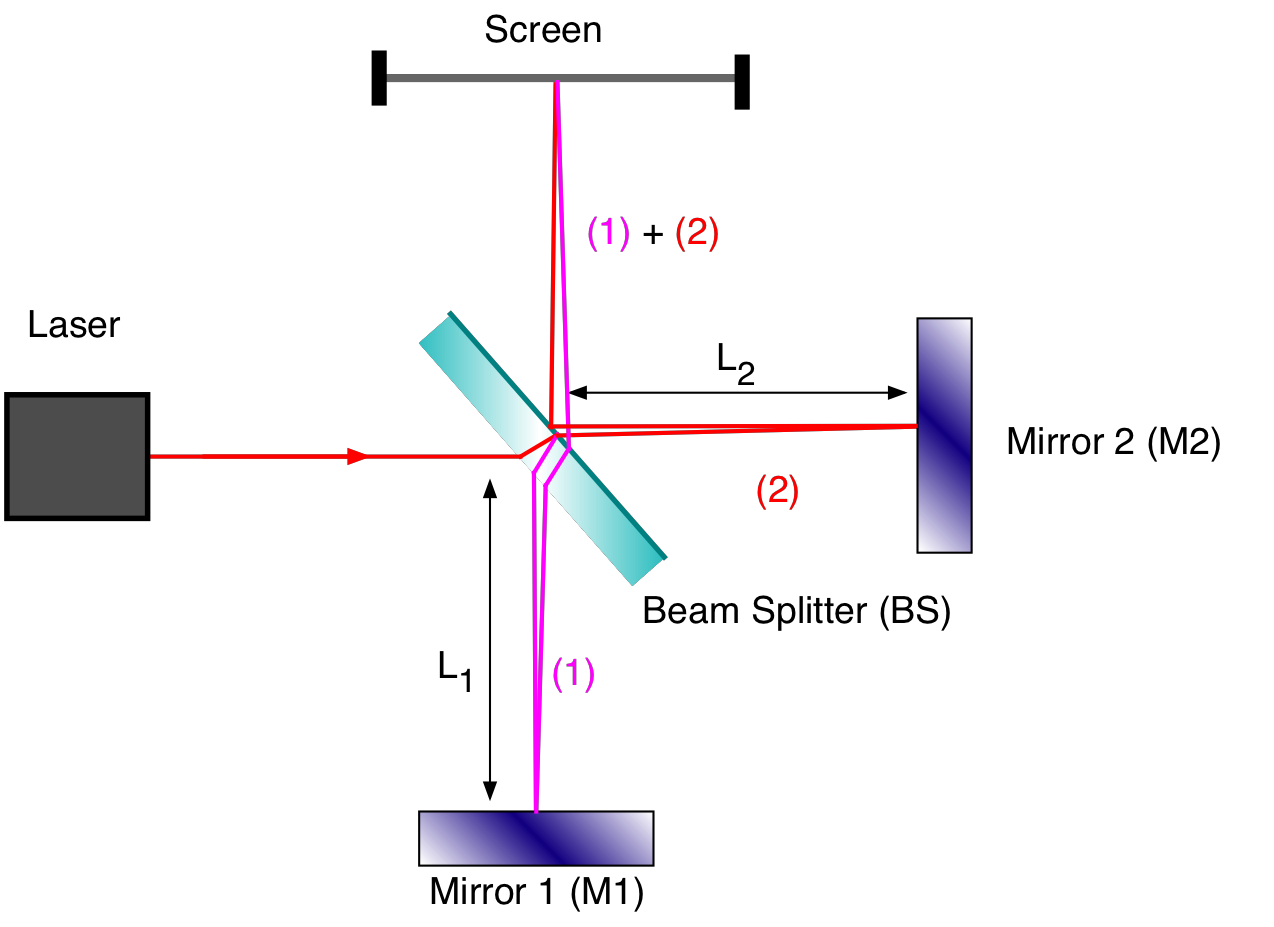
\includegraphics[width=1\textwidth]{teoria_michelson.png}
	\end{minipage}
	\begin{minipage}[c]{.40\textwidth}
	\end{minipage}
\end{center}

\begin{multicols}{2}

\section{Apparato sperimetale}

	Abbiamo a disposizione 
	\begin{itemize}
		\item Tre laser di diversa lunghezza d'onda: 633 nm (laser HeNe), 650 nm, 532 nm.
		\item Un interferometro di Michelson a divisione di ampiezza.
		\item Un motorino passo passo che mette in rotazione una vite micrometrica.
		\item Un rilevatore al silicio (fotodiodo) per misurare l'intensit� luminosa.
		\item Un piezoelettrico.
		\item Un multimetro digitale.
		\item Una camera a vuoto lunga 5 cm $\pm$ 50 $\mu$m.
		\item Una pompa a vuoto.
	\end{itemize}

\section{Misura della lunghezza d'onda}
Per misurare la lunghezza d'onda del laser contiamo le frange di interferenza al variare della differenza di cammino ottico. 

\subsection{Presa dati}
Per prima cosa allineiamo il fascio laser in modo da vedere delle frange di interferenza definite sul rilevatore al silicio. 
Al PC vediamo l'evoluzione delle frange di interferenza grazie ad un VI labVIEW, come in Figura \ref{fig:esempio_acquisizione_frange}.

\end{multicols}

\begin{figure}[H]
	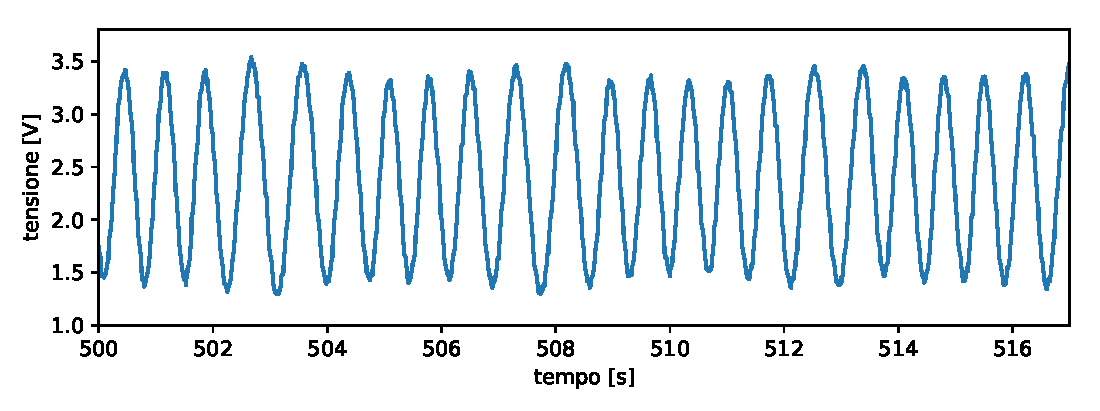
\includegraphics[width=1\textwidth]{esempio_acquisizione_frange.pdf}
	\caption{Esempio di acquisizione delle frange di interferenza.}
	\label{fig:esempio_acquisizione_frange}
\end{figure}

\begin{multicols}{2}

Al termine dell'acquisizione il VI fornisce il numero $m$ di picchi che usiamo per calcolare la lunghezza d'onda.

\subsubsection{Accorgimenti sperimentali}
\begin{itemize}
	\item Per avere un buon segnale allineiamo il fascio laser prima di inserire la lente divergente e dopo averla inserita perfezioniamo la regolazione degli specchi in modo che le frange di interferenza siano larghe in corrispondenza del rivelatore (vedi Figura \ref{fig:frange}).
	
	\item Per evitare eventuali sistematiche dovute al verso di rotazione della vite alterniamo la direzione di moto del motorino (A e B in Tabella \ref{tab:lambda}).
\end{itemize}

\begin{figure}[H]
	\centering
	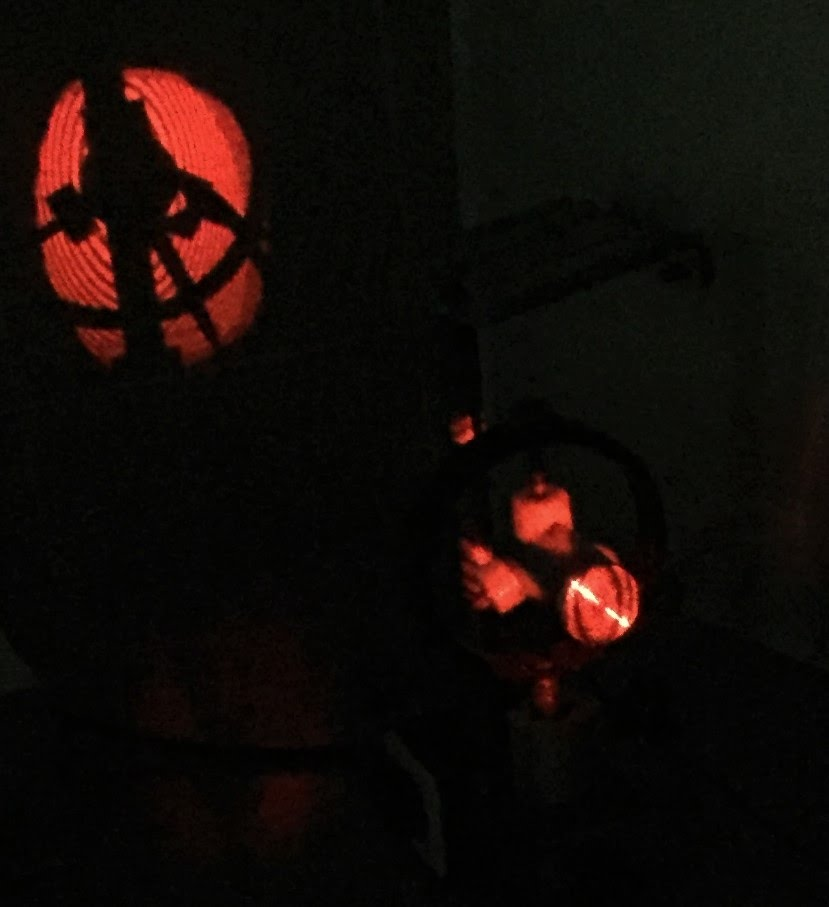
\includegraphics[width=0.3\textwidth]{frange.jpg}
	\caption{Frange di interferenza sul rilevatore.}
	\label{fig:frange}
\end{figure}

\subsection{Analisi dei dati}

\end{multicols}

\begin{table}[H]
	\centering
	\begin{tabular}{|c|ccccc|}
		\hline
		& $m(\Delta m)$ & $d(\Delta d)$ [$\mu$m] & $t$ [mm:ss] &$\lambda(\Delta\lambda)$ [nm] & direzione \\
		\hline
		\multirow{3}*{\minitab[c]{laser HeNe \\ (633 nm)}}
		& 1088(5) & 345(1) & 13:33 & 634(3) & A\\ 
		& 1094(5) &345(1) & 13:43 & 631(3) & B\\ 
		& 1092(5) &345(1) & 13:36 & 632(3) & A\\ 
		\hline
		\multirow{2}*{\minitab[c]{laser rosso \\ (650 nm)}}
		& 1065(5) &345(1) & 13:36 &  648(4) & A\\ 
		& 1054(5) &346(1) & 13:32 & 657(4) & B\\
		\hline
		\multirow{2}*{\minitab[c]{laser verde \\ (532 nm)}}
		& 1306(5) &347(1) & 13:32 & 531(3) & A\\
		& 1293(5) &347(1) & 13:32 & 537(3) & B\\
		\hline
	\end{tabular}
\caption{Dati grezzi e calcolo della lunghezza d'onda.}
	\label{tab:lambda}
\end{table}

\begin{multicols}{2}

\subsection{Conclusioni}
Per ogni laser abbiamo fatto la media dei valori di $\lambda$ misurati.
I risultati sono compatibili con quanto riportato nei datasheet. 

\begin{table}[H]
	\centering
	\begin{tabular}{|c|c|c|}
		\hline
		laser &$\lambda$ nominale [nm]& $\lambda(\Delta\lambda)$ misurata [nm]\\
		\hline
		HeNe & 632.8 & 632(2)\\
		rosso & 650 & 652(3)\\
		verde & 532 & 534(2)\\
		\hline
	\end{tabular}
\end{table}

\section{Isteresi del piezoelettrico}

In questa sezione diamo per nota $\lambda = 633$ nm e usiamo la formula $2dn = m\lambda$ per calcolare la differenza di cammino ottico $d$, ottenuta variando la tensione di alimentazione di un piezoelettrico. Eseguendo una spazzata da 0 a 100 V seguita da una da 100 a 0 V il piezoelettrico mostra un ciclo di isteresi, che andiamo ad analizzare.

\subsection{Presa dati}
Misuriamo l'alimentazione del piezoelettrico con un voltmetro collegato al PC. Il programma di acquisizione ci permette di salvare la tensione in funzione del tempo $V(t)$.
Simultaneamente avviamo il VI che conta le frange rilevate dal fotodiodo. Tramite uno script in python leggiamo il file .txt salvato dal VI ed estraiamo il tempo $t$ di ogni massimo e minimo. Infine inseriamo tali tempi nella curva $V(t)$ ottenendo un grafico $d-V$ con 2 punti ogni frangia (vedi Figura \ref{fig:esempio_acquisizione_isteresi}).

\begin{figure}[H]
	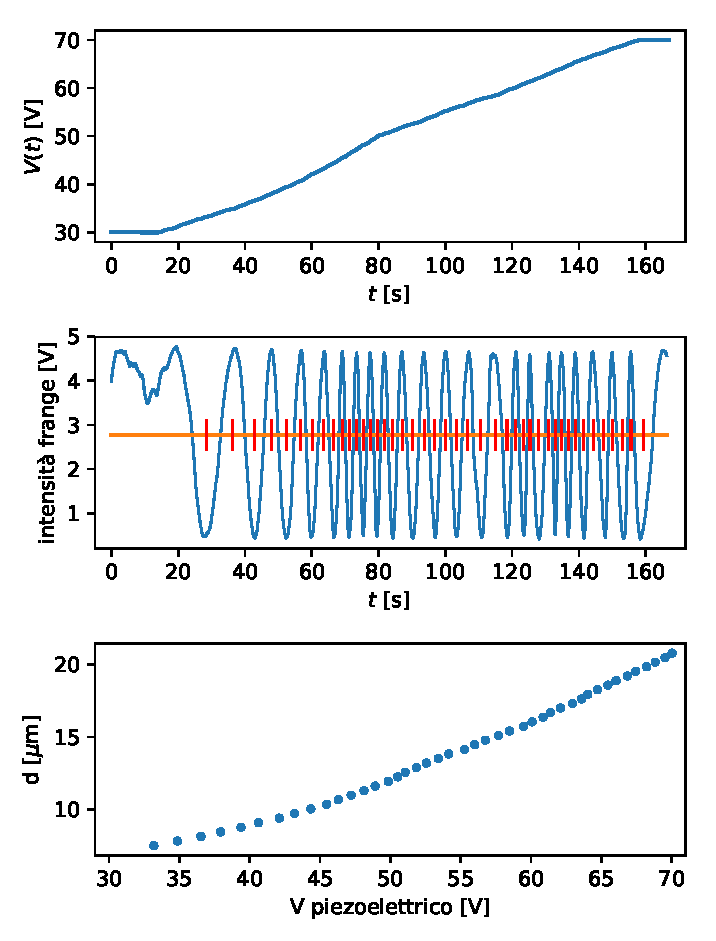
\includegraphics[width=0.5\textwidth]{esempio_acquisizione_isteresi.pdf}
	\caption{Esempio di acquisizione della curva del piezoelettrico.}
	\label{fig:esempio_acquisizione_isteresi}
\end{figure}

\subsection{Analisi dati}

\subsubsection{Alimentazione da 0 a 100 Volt}
L'errore sull'alimentazione � dato dalla fluttuazione del valore letto al multimetro (0.2 V) mentre l'errore su $d$ � la distanza tra due frange.

\end{multicols}

\begin{figure}[H]
	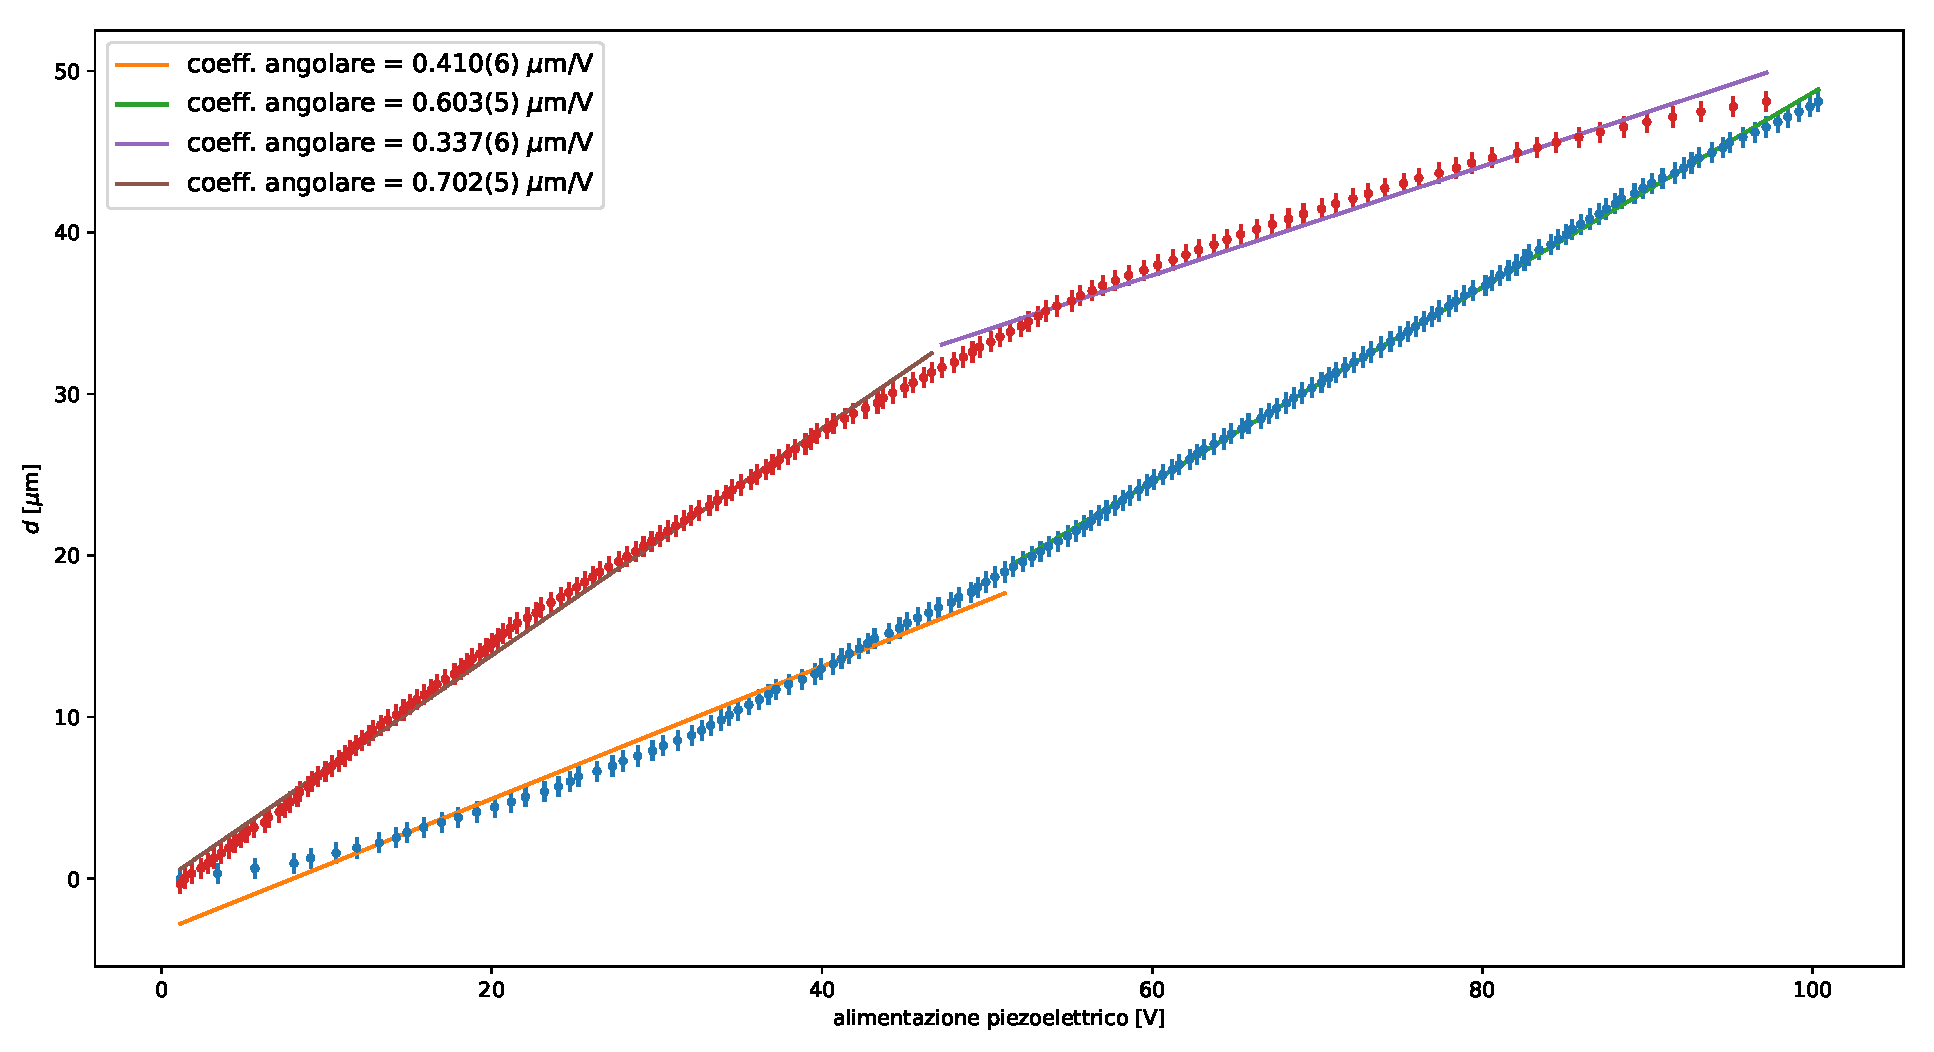
\includegraphics[width=1\textwidth]{isteresi_0-100.pdf}
	\caption{Isteresi del piezoelettrico: 0-100 V.}
	\label{fig:0-100}
\end{figure}

\begin{multicols}{2}

\subsubsection{Alimentazione da 30 a 70 Volt}

\end{multicols}

\begin{figure}[H]
	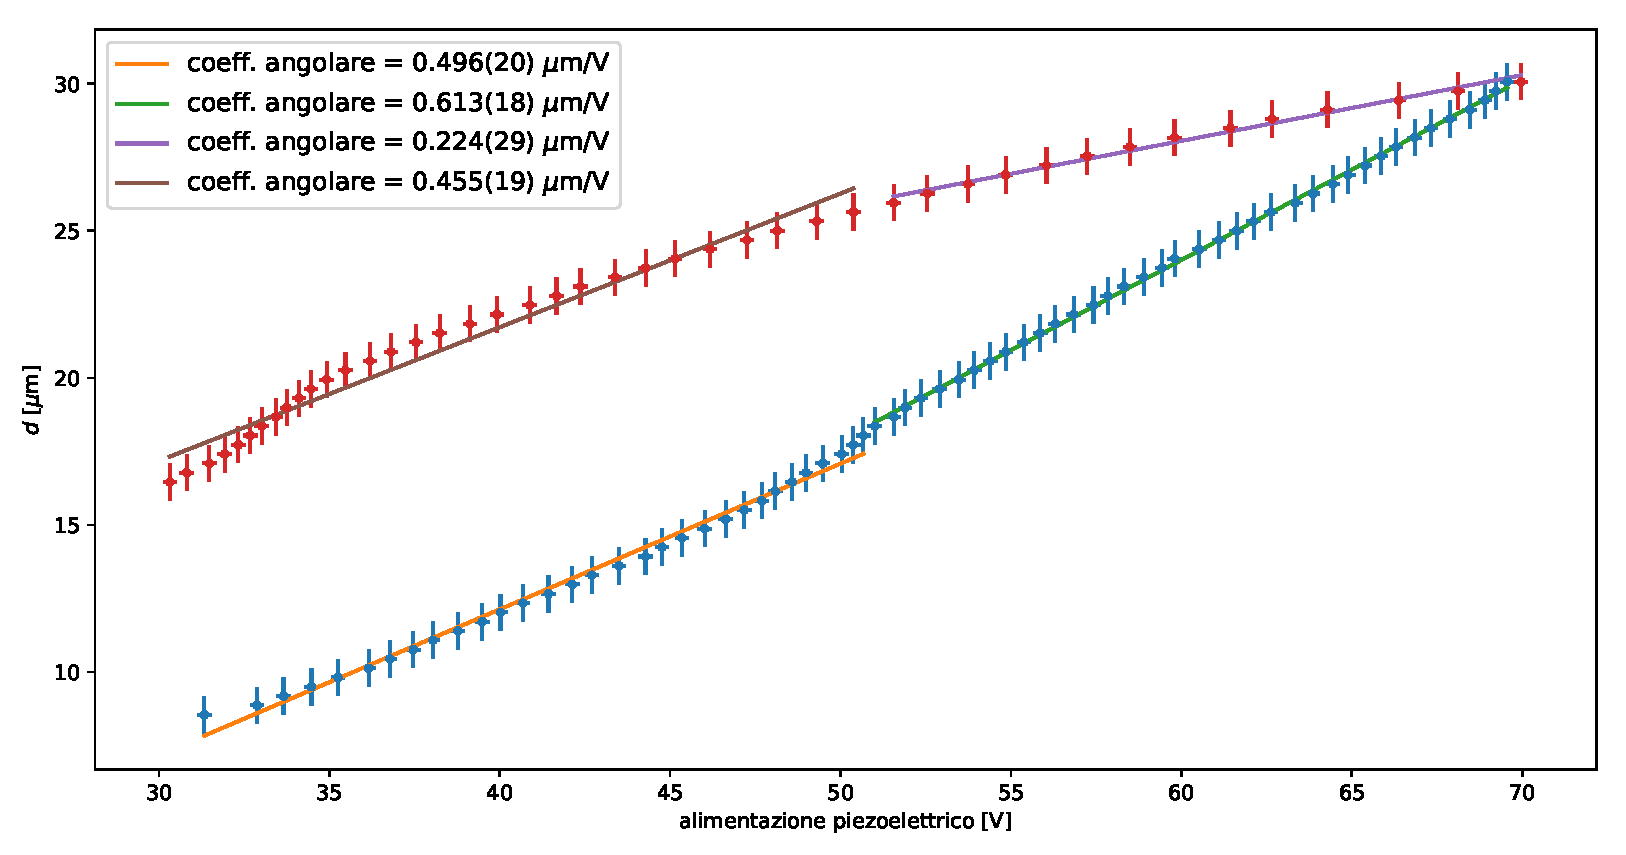
\includegraphics[width=1\textwidth]{isteresi_30-70-1.pdf}
	\caption{Isteresi del piezoelettrico: 30-70 V.}
	\label{fig:30-70-1}
\end{figure}

\begin{multicols}{2}

 
 \end{multicols}
 
 \begin{figure}[H]
 	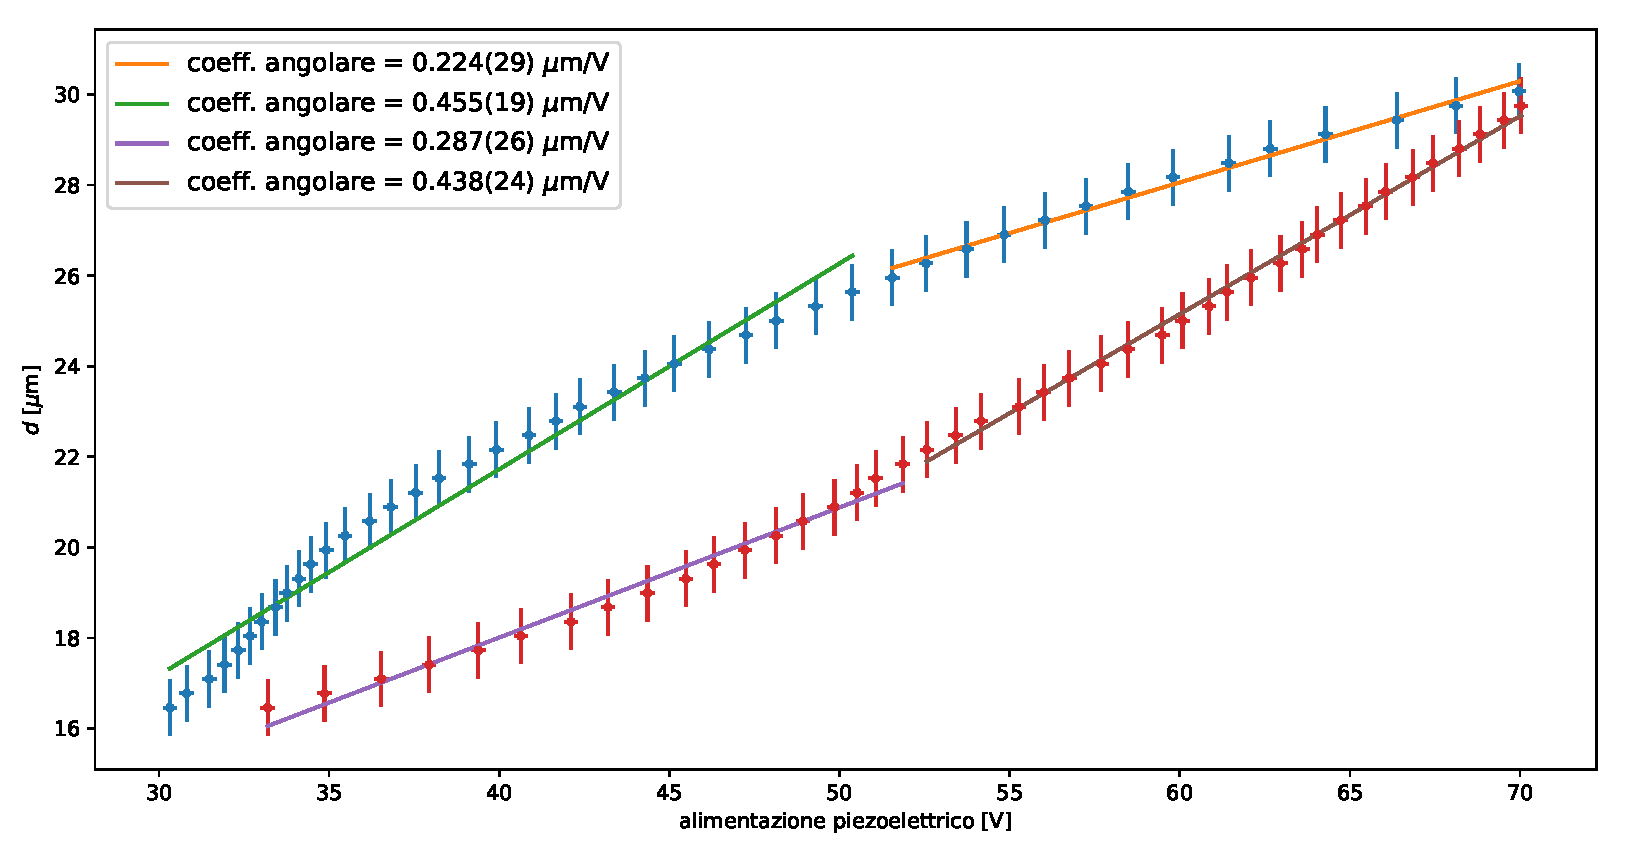
\includegraphics[width=1\textwidth]{isteresi_30-70-2.pdf}
 	\caption{Isteresi del piezoelettrico: 30-70 V.}
 	\label{fig:30-70-2}
 \end{figure}
 
 \begin{multicols}{2}

\subsection{Conclusioni}

\section{Indice di rifrazione dell'aria}

Utilizziamo adesso l'interferometro di Michelson per misurare l'indice di rifrazione di un mezzo in cui si propaga la luce laser nota la sua lunghezza d'onda e la distanza percorsa dal fascio nel mezzo. 

\subsection{Acquisizione dati}

\subsection{Analisi dati}
\begin{equation}
\Delta n = \frac{m\lambda}{2d}
\end{equation}



\begin{table}[H]
	\centering
	\begin{tabular}{|c|c|c|c|}
		\hline
		laser & $\lambda$ & frange  & $n(\Delta n)$ \\
		\hline
		HeNe & 632.8 & 43(1) &1.000272(6)\\
		rosso & 650 & 41(1) &1.000267(7)\\ 
		verde & 532 & 51(1) &1.000271(5)\\
		\hline
	\end{tabular}
	\caption{Indice di rifrazione dell'aria}
	\label{tab:n}
\end{table}

\end{multicols}


\end{document}
